

\begin{figure}[t]
  \captionsetup[subfigure]{justification=centering}
  \centering
  \begin{subfigure}{0.048\linewidth}
    \centering
    \includegraphics[width=\linewidth]{plots/xlegend.pdf}
    \begin{minipage}{.1cm}
      \vfill
    \end{minipage}
  \end{subfigure}%
  \begin{subfigure}{0.29\linewidth}
    \centering
    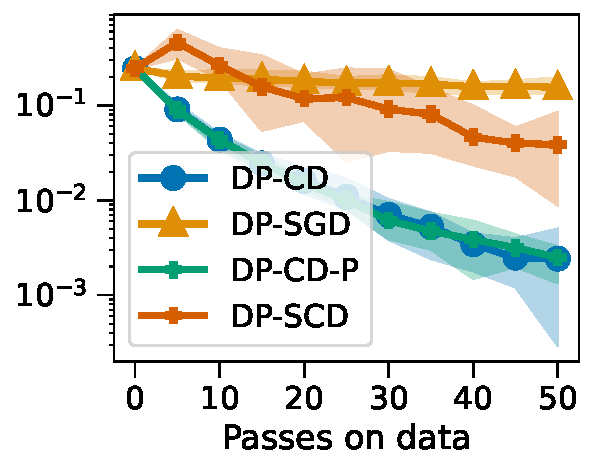
\includegraphics[width=\linewidth]{plots/optimization_electricity_raw.pdf}
    \caption{Electricity\\ Logistic, $\lambda=1/n$.}
    \label{fig:expe-logreg-constant}
  \end{subfigure}%
  \begin{subfigure}{0.29\linewidth}
    \centering
    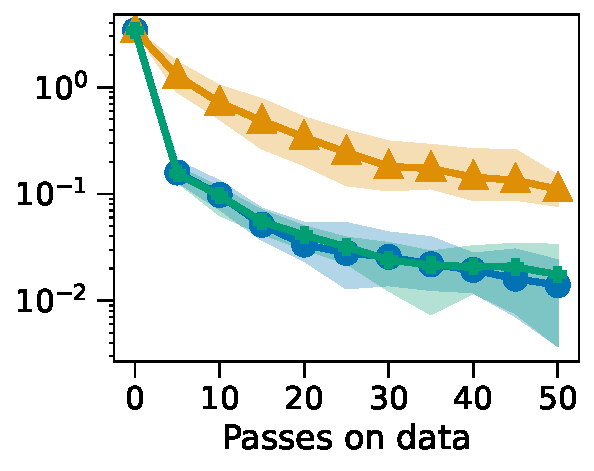
\includegraphics[width=\linewidth]{plots/optimization_california_raw.pdf}
    \caption{California\\ LASSO, $\lambda=1.0$.}
    \label{fig:expe-logreg-power-law-sparse}
  \end{subfigure}

  \caption{ Relative error to non-private optimal for DP-CD (blue), DP-CD with
  privately estimated coordinate-wise smoothness
    constants (green), DP-SGD (orange) and DP-SCD (red, only applicable to the
    smooth case) on
    two \emph{imbalanced} problems. The number of passes is
    tuned separately for each algorithm to achieve lowest error. We report
    min/mean/max values over 10~runs.}
  \label{fig:expe-raw}
\end{figure}

\section{Numerical Experiments}
\label{sec:numerical-experiments}


In this section, we assess the practical performance of DP-CD against
(proximal) DP-SGD on LASSO\footnote{\ie
  $\ell(w, (x,y)) = (w^\top x - y)^2$, $\psi(w) = \lambda\norm{w}_1$.}
and $\ell_2$-regularized logistic regression\footnote{\ie
  $\ell(w, (x, y)) = \log(1 + \exp(-y w^\top x))$,
  $\psi(w) = \!\frac{\lambda}{2}\!\norm{w}_2^2$.}. On the latter
problem, we also consider the dual private coordinate
descent algorithm of \citet{damaskinos2021Differentially}
(DP-SCD). For LASSO, we use the California dataset
\citep{kelleypace1997Sparse}, with $n=20,640$ records and $p=8$
features as well as a synthetic dataset (coined ``Sparse LASSO'') with
$n=1,000$ records and $p=1,000$ independent features that follow a
standard normal distribution.  The labels are then computed as a noisy
sparse linear combination of a subset of $10$ active features.  For
logistic regression, we consider the Electricity dataset
\citep{Electricity} with $45,312$ records and $8$ features.  On
California and Electricity, we set $\epsilon=1$ and $\delta=1/n^2$,
which is generally seen as a rather high privacy regime. The Sparse
LASSO dataset corresponds to a challenging setting for privacy
($n=p$), so we consider a low privacy regime with $\epsilon=10$,
$\delta=1/n^2$.  Privacy accounting for DP-SGD is done by numerically
evaluating the Rényi DP formula given by the sampled Gaussian
mechanism \citep{mironov2019Enyi}. Similarly for DP-CD, we do not use
the closed-form formula of Theorem~\ref{thm:dp-cd-privacy} but rather
numerically evaluate the tighter Rényi DP formula given in
Appendix~\ref{sec:proof-privacy}.

For DP-SGD, we use constant step sizes and standard gradient
clipping. For DP-CD, we adapt the coordinate-wise clipping thresholds
from one hyperparameter, as described in
\Cref{sub:clipping}. Similarly, coordinate-wise step sizes are set to
$\gamma_j = \gamma / M_j$, where $\gamma$ is a hyperparameter. When
the coordinate-wise smoothness constants are not all equal, we also
consider DP-CD with privately computed $M_j$'s, as described in
\Cref{sec:priv-smoothn}.  For each dataset and each algorithm, we
simultaneously tune the clipping threshold, the number of passes over
the dataset and, for DP-CD and DP-SGD, the step sizes.  After tuning
these parameters, we report the relative error to the (non-private)
optimal objective value.  The complete tuning procedure is described
in \Cref{sec:hyperp-tuning}, where we also give the best error for
various numbers of passes for each algorithm and dataset.  The code
used to obtain all our results is available in a public repository\footnote{
\url{https://gitlab.inria.fr/pmangold1/private-coordinate-descent/}}
and in the supplementary material.

\subsection{Imbalanced Datasets}
\label{sec:raw-datasets}


In the Electricity and California datasets, features are naturally
imbalanced. DP-CD can exploit this through the use of coordinate-wise
smoothness constants. We also consider a variant of DP-CD (DP-CD-P)
which dedicates $10\%$ of the privacy budget~$\epsilon$ to estimate
these constants (see \Cref{sec:priv-smoothn}) from a crude upper bound
on each feature (twice their maximal absolute value). It then uses the
resulting private smoothness constants in step sizes and clipping
thresholds. \Cref{fig:expe-raw} shows that DP-CD outperforms DP-SGD
and DP-SCD by an order of magnitude on both datasets, even when the
smoothness constants are estimated privately.



\subsection{Balanced Datasets}
\label{sec:stand-datas}

To assess the performance of DP-CD when coordinate-wise smoothness
constants are balanced, we standardize the Electricity and California
datasets (see Section~\ref{sec:data-standardization}).  As
standardization is done for all algorithms, we do not account for it
in the privacy budget. On standardized datasets, coordinate-wise
smoothness constants are all equal, removing the need of estimating
them privately. We report the results in \Cref{fig:expe-standardized}.
Although our theory suggests that DP-CD may do worse than DP-SGD in
balanced regimes, we observe that it still improves over DP-SGD (and
DP-SCD) in practice. Similar observations hold in our challenging
Sparse LASSO problem, where DP-SGD is barely able to make any
progress. We believe these results are in part due to the beneficial
effect of clipping in DP-CD, and the fact that DP-SGD relies on
amplification by subsampling, for which privacy accounting is not
perfectly tight. Additionally, CD methods are known to perform well on
fitting linear models: our results show that this transfers well to
private optimization.

\begin{figure*}[t]
  \captionsetup[subfigure]{justification=centering}
  \centering
  \begin{subfigure}{0.048\linewidth}
    \centering
    \includegraphics[width=\linewidth]{plots/xlegend.pdf}
    \begin{minipage}{.1cm}
      \vfill
    \end{minipage}
  \end{subfigure}%
  \begin{subfigure}{0.29\linewidth}
    \centering
    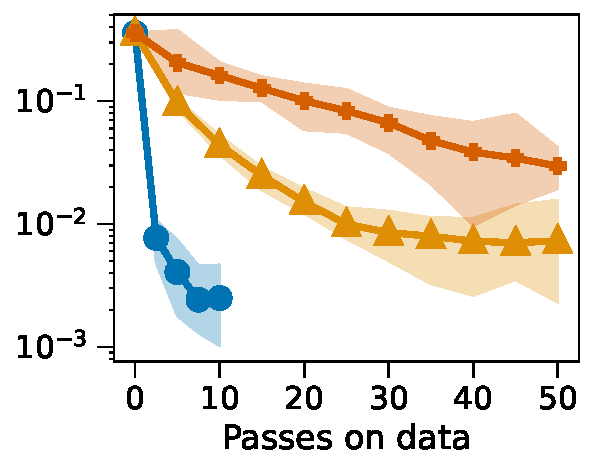
\includegraphics[width=\linewidth]{plots/optimization_electricity_norm.pdf}
    \caption{Electricity\\ Logistic, $\lambda=1/n$.}
    \label{subfig:expe-logreg-constant}
  \end{subfigure}%
  \begin{subfigure}{0.29\linewidth}
    \centering
    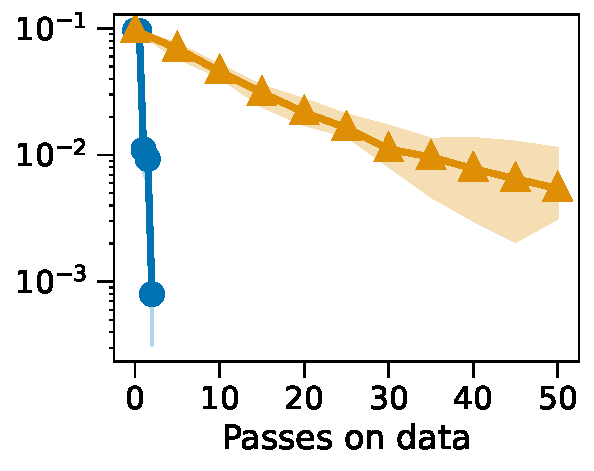
\includegraphics[width=\linewidth]{plots/optimization_california_norm.pdf}
    \caption{California\\ LASSO, $\lambda=0.1$.}
    \label{subfig:expe-logreg-power-law}
  \end{subfigure}
  \begin{subfigure}{0.29\linewidth}
    \centering
    \includegraphics[width=\linewidth]{plots/optimization_lasso.pdf}
    \caption{Sparse\\ LASSO, $\lambda=30$.}
    \label{fig:expe-logreg-power-law}
  \end{subfigure}

  \caption{
    Relative error to non-private optimal for  DP-CD (blue), DP-SGD (orange)
    and DP-SCD (red, only applicable to the smooth case) on three
    \emph{balanced} problems. The number of passes is tuned separately for
    each algorithm to achieve lowest error. We report min/mean/max values over
    10~runs.
  }
  \label{fig:expe-standardized}
\end{figure*}

\subsection{Running Time}
\label{sec:running-time}

The results above showed that DP-CD yields better
utility than DP-SGD. We also observe that DP-CD tends to reach
these
results in up to $10$~times fewer passes on the data than DP-SGD (see
\Cref{sec:hyperp-tuning} for detailed results). Additionally, when accounting
for running time, DP-CD
significantly outperforms DP-SGD: we refer to \Cref{sec:running-time-in} for
the counterparts of \Cref{fig:expe-raw} and \ref{fig:expe-standardized} as a
function of the running time instead of the number of passes.



























